\documentclass{article}
\usepackage[utf8]{inputenc}
\usepackage{amsmath}
\usepackage{amsfonts}
\usepackage{geometry}
\usepackage{stmaryrd}
\usepackage[table]{xcolor}
\usepackage{fancybox}
\usepackage{tikz}
\usepackage{listings}
\usepackage{adjustbox}
\usetikzlibrary{positioning}
\geometry{a4paper,left=25mm,right=25mm,top=20mm}

\title{Planification du pompage dans un réseau de distribution d'eau potable ramifié\\-\\Optimisation non-linéaire en nombre entier}
\author{Robinson Beaucour}
\date{Décembre 2022}

\begin{document}

\maketitle

\begin{figure}[h]
    \centering
    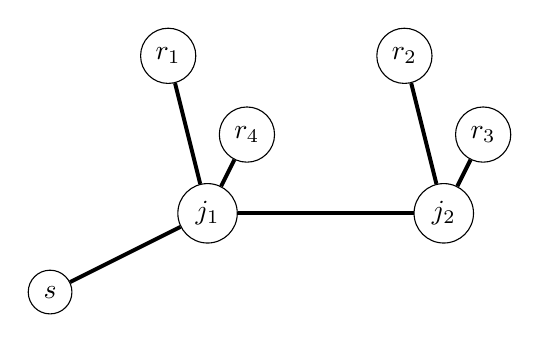
\begin{tikzpicture}[main/.style = {draw, circle}] 
        \node[main] (s) at (0,0) {$s$};
        \node[main] (j_1)   at (2,1)    {$j_1$}; 
        \node[main] (j_2)   at (5,1)    {$j_2$};
        \node[main] (r_1)   at (1.5,3)  {$r_1$};
        \node[main] (r_4)   at (2.5,2)  {$r_4$};
        \node[main] (r_2)   at (4.5,3)  {$r_2$};
        \node[main] (r_3)   at (5.5,2)  {$r_3$};
        \draw   [line width=0.5mm]  (s)     --  (j_1);
        \draw   [line width=0.5mm]  (j_1)   --  (j_2);
        \draw   [line width=0.5mm]  (j_1)   --  (r_1);
        \draw   [line width=0.5mm]  (j_1)   --  (r_4);
        \draw   [line width=0.5mm]  (j_2)   --  (r_2);
        \draw   [line width=0.5mm]  (j_2)   --  (r_3);
    \end{tikzpicture}
    \caption{Réseau de distribution simple}
\end{figure}

\paragraph{Variables de décision}
$$
\left.
    \begin{array}{lll}
        Q_{pompe,t}^{(k)}       &   \text{Débit sortant de la pompe $k$ à l'instant $t$} & \mathbb{R}_+\\[0.2cm]
        Q_{reserv,t}^{(r)}      &   \text{Débit entrant du réservoire $r$ à l'instant $t$}& \mathbb{R}_+\\[0.2cm]
        P_{pompe,t}^{(k)}       &   \text{Puissance électrique consommée par la pompe $k$ à l'instant $t$}& \mathbb{R}_+\\[0.2cm]
        V_t^{(r)}               &   \text{Volume du réservoire $r$ à l'instant $t$}& [V_{min}^{(r)},V_{max}^{(r)}]\\[0.2cm]
        N_{on,t}^{(k)}          &   \text{Etat de la pompe $k$ (allumé/éteint) à l'instant $t$}&\{0,1\}\\[0.2cm]
    \end{array}
\right.
$$
\paragraph{Contraintes}
$$
\left.
    \begin{array}{lcccc}
        \forall t   &   \sum_k Q_{pompe,t}^{(k)}    & = &   \sum_r Q_{reserv,t}^{(r)}  &   \text{Equilbre débit sur le réseau}\\[0.2cm]
        \forall t   &   V_{t+1}^{(r)}-V_t^{(r)}     & = &   Q_{reserv,t}^{(r)} - D_t^{(r)} & \text{Satisfaction de la demande (pas horaire)}\\[0.2cm]
        \forall k,t &   P_{pompe,t}^{(k)}           & = &   \psi_0^{(k)}N_{on,t}^{(k)}  + \psi_2^{(k)}(Q_{pompe,t}^{(k)})^2 &   \text{Fonctionnement pompe}\\[0.2cm]
    \end{array}
\right.
$$
\begin{adjustbox}{max width=\textwidth}
    \begin{lstlisting}
        Noeud(t) ..                   sum(k, Qpompe(k,t)) =e=  sum(r, Qreserve(r,t));
        Satisfaction_demande(r,t) ..  v(r,t+1) - v(r,t)   =e=  1 * (Qreserve(r,t)-demand(r,t));
        Elec_pompe(k,t) ..            Ppompe(k,t)         =e=  psi("small","0") * Non(k,t) +psi("small","2") * Qpompe(k,t)**2;
        obj ..                        z                   =e=  sum((k,t), Ppompe(k,t)*tariff(t));
    \end{lstlisting}
\end{adjustbox}

\paragraph{Objectif}
$$
    \text{Minimiser }   \sum_t \sum_k P_{pompe,t}^{(k)}\cdot C_t
$$
\end{document}
